\chapter{Gestión del proyecto}
\label{sec:gestion}

\section{Alcance}

\subsection{Descripción del alcance del proyecto}

En este proyecto se construirá un módulo software como parte del proyecto Pyomo. Este nuevo módulo adaptará el funcionamiento del actual módulo de programación estocástica (\textit{PySP}) a una implementación paralela.\\

Se realizará un estudio inicial de Pyomo para decidir la integración y la tecnología a utilizar para la nueva implementación. El objetivo de esta nueva implementación es el de proporcionar una ejecución más escalable que permita abordar problemas de mayor tamaño o, al menos, proporcionar una implementación base que, con futuras optimizaciones, permita conseguir ese objetivo.\\

El rendimiento de esta nueva implementación estará reflejado en un informe tras hacer pruebas con distintos problemas y en distintos sistemas.

\subsection{Criterios de aceptación}

El proyecto será aceptado cuando se superen las pruebas definidas en \autoref{sec:pruebas}.\\

El proyecto persigue dos objetivos: la implementación del algoritmo en paralelo y un estudio de rendimiento. La intención es buscar una implementación alternativa y estudiar su viabilidad, no es necesario que la nueva implementación sea inicialmente mejor que la anterior.

\subsection{Entregables del proyecto}

Los elementos a entregar tras la finalización del proyecto son:

\begin{itemize}
    \item Código de Pyomo actualizado con el módulo de ejecución de PH paralelo.
    \item Estudio de rendimiento (incluído en el documento actual).
    \item Memoria de realización del proyecto.
    \item Otra documentación asociada a la realización del proyecto.
\end{itemize}

\subsection{Exclusiones}

El proyecto producirá una implementación paralela del algoritmo PH existente. Esta implementación debe ser funcional pero no es un objetivo del proyecto hacer que esta nueva implementación sea mejor que la anterior en términos de eficiencia o rapidez.

\subsection{Restricciones}

El proyecto debe finalizar el día 18/06/2018. En caso de ser necesario se puede postponer la fecha de finalización hasta el 27/07/2018.

\section{Análisis de requisitos}

El objetivo principal de este trabajo es el de paralelizar el algoritmo Progressive Hedging del módulo PySP. Para conseguirlo se establecen los siguientes requisitos:

\Req [
    id=RF-01,
    name={Ejecución de trabajos en Spark},
    description={Ejecutar el algoritmo PH en Spark de forma paralela.},
    priority={Imprescindible}
]

\Req [
    id=RF-02,
    name={Integración con Pyomo},
    description={La solución implementada debe funcionar como parte del programa Pyomo.},
    priority={Imprescindible}
]

\Req [
    id=RF-03,
    name={Interoperabilidad con funcionalidad previa},
    description={La nueva implementación no debe impedir el correcto funcionamiento de los módulos de Pyomo existentes.},
    priority={Importante}
]

\Req [
    id=RF-04,
    name={Establecer medición de rendimiento de Spark},
    description={Cuantificar la diferencia de rendimiento y escalabilidad de la nueva implementación.},
    priority={Importante}
]

\section{Análisis de riesgos}

Para un proyecto del tamaño y duración estimados para este TFG es de vital importancia analizar los posibles riesgos que pueden poner en peligro la satisfactoria finalización del trabajo.\\

A continuación se especifican los potenciales riesgos junto a su probabilidad, impacto y tratamiento.\\

La probabilidad se medirá como:

\begin{itemize}
    \item \textbf{Muy alta:} Probabilidad de ocurrencia superior al 90\%.
    \item \textbf{Alta:} Probabilidad de ocurrencia superior al 70\%.
    \item \textbf{Moderada:} Probabilidad de ocurrencia superior al 40\%.
    \item \textbf{Baja:} Probabilidad de ocurrencia inferior al 40\%.
\end{itemize}

El impacto que tendrá la ocurrencia del riesgo sobre los activos afectados se medirá como:

\begin{itemize}
    \item \textbf{Catastrófico: } Supone la cancelación de tareas, inhabilidad de cumplir la fecha límite o, por último, la cancelación del trabajo.
    \item \textbf{Serio: } Supone modificaciones importantes pero asumibles en la realización de las tareas o el tiempo asignado a las mismas.
    \item \textbf{Tolerable: } La aparición del riesgo causará la necesidad de trabajo extra pero asumible. También puede suponer eliminar tareas o resultados poco importantes.
    \item \textbf{Irrelevante: } Las consecuencias generadas por el riesgo pueden ignorarse sin efectos demasiado negativos.
\end{itemize}

\RiskItem [
    id={R-01},
    name={Mala gestión del tiempo de realización del anteproyecto},
    description={
        Un anteproyecto erróneo puede suponer el rechazo del mismo. En menor medida, una descripción demasiado concreta puede suponer un limitante a la hora de realización del trabajo.
    },
    probability={Moderada},
    impact={Catastrófico},
    affected={Anteproyecto},
    treatment={Prevención -- Generar una lista de elementos necesarios para el anteproyecto, planificarlos temporalmente y cumplir dicha planificación.},
    indicators={No cumplir la planificación.},
    follow={Semanal.}
]

\RiskItem [
    id={R-02},
    name={No identificar correctamente los objetivos del trabajo},
    description={
        Unos objetivos poco claros pueden llevar a realizar trabajo innecesario o no realizar trabajo imprescindible. También pueden ocasionar desarrollo más lento por no saber qué hacer a continuación.
    },
    probability={Moderada},
    impact={Serio},
    affected={Anteproyecto, Planificación temporal, Código},
    treatment={Minimización -- Revisión de los objetivos dispuestos en el anteproyecto con el tutor del TFG. Esta revisión se hará con antelación suficiente para realizar cambios si fuesen necesarios.},
    indicators={Redacción poco clara del propósito del trabajo en la realización del anteproyecto.},
    follow={Semanal.}
]

\RiskItem [
    id={R-03},
    name={Inhabilidad para ajustar el trabajo a las horas requeridas},
    description={
        La realización de un TFG tiene establecida una cantidad de horas fija. Su incumplimiento debe estar justificado.
    },
    probability={Alta},
    impact={Tolerable},
    affected={Planificación temporal},
    treatment={Minimización -- Se estimará la duración de las tareas al alza. En caso de que la planificación acabé con más horas de las permitidas, se podrá disminuir la duración de las tareas menos importantes.},
    indicators={La planificación suma más horas de las permitidas.},
    follow={Cada vez que se modifique la planificación.}
]

\RiskItem [
    id={R-04},
    name={Memoria final poco concreta},
    description={
        La memoria del proyecto debe representar fielmente el desarrollo del mismo. Si se retrasa demasiado su realización es posible perder detalles relevantes del proyecto.
    },
    probability={Alta},
    impact={Serio},
    affected={Memoria},
    treatment={Minimización -- Se realizarán, semanalmente o cada 15 días, documentos de progreso que especifiquen las tareas realizadas. Con esto se tendrá una documentación informal pero muy actualizada y concreta.},
    indicators={Parte del desarrollo no está especificado en ningún documento de progreso ni en la memoria final.},
    follow={Semanalmente.}
]

\RiskItem [
    id={R-05},
    name={Incumplimiento del cronograma del proyecto},
    description={
        Por errores de código, inexperiencia o una carga de trabajo externa mayor de lo esperada, algunas tareas pueden durar más de lo planificado.
    },
    probability={Muy alta},
    impact={Serio},
    affected={Planificación temporal},
    treatment={Prevención -- Seguir el porcentaje de cumplimiento de las tareas sobre el cronograma.},
    indicators={Una tarea no se finaliza en plazo o el porcentaje de realización no es suficiente para el tiempo establecido en la tarea.},
    follow={Diario.}
]

\RiskItem [
    id={R-06},
    name={Incompatibilidad de la herramienta escogida con Pyomo},
    description={
        Se hará un estudio de herramientas para paralelizar el algoritmo. Si esta herramienta sufre algún tipo de incompatibilidad con el proyecto existente supondrá un retraso importante.
    },
    probability={Baja},
    impact={Catastrófico},
    affected={Diseño, Código},
    treatment={Prevención -- Durante la elección de la herramienta se harán pruebas sencillas sobre el proyecto. Tras crear el diseño se hará una implementación de prueba.},
    indicators={Aparecen errores en el programa que no son causados por fallos de programación.},
    follow={Semanal durante la fase de diseño. Cada 15 días durante la implementación.}
]

\RiskItem [
    id={R-07},
    name={Retraso del proyecto},
    description={
        Alguna de las tareas planificadas dura más de lo especificado. El impacto dependerá de la gravedad del retraso.
    },
    probability={Moderada},
    impact={Variable},
    affected={Todos los ECS},
    treatment={Minimización -- La planificación se creará con un margen de retraso proporcional a la complicación de la tarea.},
    indicators={Una tarea está tardando en finalizar más de lo esperado.},
    follow={Semanalmente.}
]

\RiskItem [
    id={R-08},
    name={No conseguir acceso a un cluster},
    description={
        Para probar el software es ideal utilizar un cluster de computación que permita evaluar la escalabilidad de la solución.
    },
    probability={Moderada},
    impact={Serio},
    affected={Memoria, Informe de rendimiento},
    treatment={Aceptar -- La pruebas se realizarán en un ordenador personal y es posible que tengan resultados menos relevantes.},
    follow={Al finalizar la implementación y al comenzar la ejecución de las pruebas.}
]

\section{Análisis de costes}

En esta sección se realizará un cálculo de los costes del proyecto basados en la planificación temporal establecida.\\

\subsection{Costes materiales}

En primer lugar se hará un cálculo de los costes materiales necesarios para la realización del proyecto.

El único material utilizado ha sido el ordenador de desarrollo. Considerando una vida útil de 4 años y un precio base de 800{\euro} el precio de su uso a lo largo de 78 días es:

\begin{equation}
    \frac{800}{365*4} * 78 = 42\mbox{\euro}
\end{equation}

Todo el software utilizado para la realización del proyecto es gratuito a excepción de MSProject, del cual se hizo uso de la licencia de prueba gratuita.

\subsection{Costes personales}

El coste del desarrollador se estima en 16.300{\euro} brutos. Deduciendo IRPF y costes de Seguridad social, se estima el coste por hora en 9{\euro}.\\

Se deben tener en cuenta los gastos que suponen las reuniones con el tutor del TFG. Se calcula un coste por hora de 20{\euro} y un tiempo total de reuniones en 25h.\\

Si el proyecto dura 78 días y está planificado para un trabajo diario de 5h, los costes personales son:\\

\begin{tabularx}{\linewidth}{|p{3cm}|X|}
    \hline
    \textbf{Desarrollador} & $9*78*5=3510\mbox{\euro}$ \tabularnewline
    \hline
    \textbf{Tutor} & $20*25=500\mbox{\euro}$ \tabularnewline
    \hline
\end{tabularx}

\subsection{Costes indirectos}

Estos costes no están directamente relacionados con el desarrollo del proyecto pero proveen bienes necesarios para la realización del mismo. Entre ellos se encuentran servicios básicos como electricidad e internet.\\

Durante la realización del proyecto se hace uso de estos servicios proporcionados por la universidad mediante el Servicio Universitario de Residencias. \\

Considerando que el proyecto supone 5h diarias, esto es un 13\% del tiempo de uso de dichos servicios. Por lo tanto, en 5 meses (teniendo en cuenta la realización del anteproyecto): 29,25{\euro}

\subsection{Costes tras la ampliación del proyecto}

Una vez modificada la fecha de finalización del proyecto contamos con un mes adicional de gastos. Este nuevo mes debe contar con nuevos gastos indirectos por residir en la vivienda personal, lo que también implica un coste de 10{\euro} por cada reunión que suponga un desplazamiento a Santiago.\\

Esta nueva fecha de finalización supone 40 días extra de gasto. \\

En cuanto a costes materiales, se sumarán 40 días al uso del ordenador, sumando 22{\euro} extra.\\

Los gastos personales, asumiendo otras 15h extra para el tutor:\\

\begin{tabularx}{\linewidth}{|p{3cm}|X|}
    \hline
    \textbf{Desarrollador} & $9*40*5=1800\mbox{\euro}$ \tabularnewline
    \hline
    \textbf{Tutor} & $20*15=300\mbox{\euro}$ \tabularnewline
    \hline
\end{tabularx}
\ \\
En los gastos indirectos, el precio ahora es superior, contando 57{\euro} de conexión a internet a mayores del resto de facturas, manteniendo el 13\% de uso, suma otros 90{\euro} en los meses de Junio y Julio.\\

Adicionalmente, se consideran 3 reuniones en este periodo adicional, con un coste de 13{\euro} cada una.

\subsection{Resumen de costes}
\ \\
\begin{tabularx}{\linewidth}{|p{3cm}|X|}
    \hline
    \textbf{Personales} & 6110{\euro} \tabularnewline
    \hline
    \textbf{Materiales} & 64{\euro} \tabularnewline
    \hline
    \textbf{Indirectos} & 158,25{\euro} \tabularnewline
    \hline
\end{tabularx}
\ \\
De esta forma determinamos un \textbf{coste total del proyecto} de 6332,25{\euro}

\section{Gestión de la configuración}

Para especificar la Gestión de la Configuración de este proyecto primero debemos identificar los Elementos de Configuración de Software (ECS), es decir, los elementos que se verán afectados por esta Gestión de la Configuración.\\

Elementos de Configuración:
\begin{itemize}
    \item Proyecto de software.
    \item Memoria del proyecto.
    \item Anteproyecto.
    \item Documentos de análisis y diseño.
    \item Informes de progreso.
    \item Plantillas de documentos.
\end{itemize}

Para gestionar las diferentes versiones de estos elementos de configuración se creará un repositorio git alojado en Github. Este repositorio contendrá toda la documentación. Para añadir el proyecto de software se realizará un \textit{fork} del proyecto Pyomo original y se añadirá como un submódulo a nuestro repositorio base. \\

Las modificaciones sobre el software serán individuales por lo que no será necesario considerar técnicas de consistencia en trabajo colaborativo. Para los cambios que se realicen se crea una rama específica sobre el \textit{fork} del proyecto.\\

Para relacionar de forma concreta tareas de la planificación con cambios en el repositorio se utiliza un tablero en la plataforma \textit{Trello}. Estas tareas se reflejan en los informes de progreso del repositorio. Además, funciona como herramienta organizativa.

\section{Planificación temporal}

\subsection{EDT}

\begin{figure}[H]
    \centerline{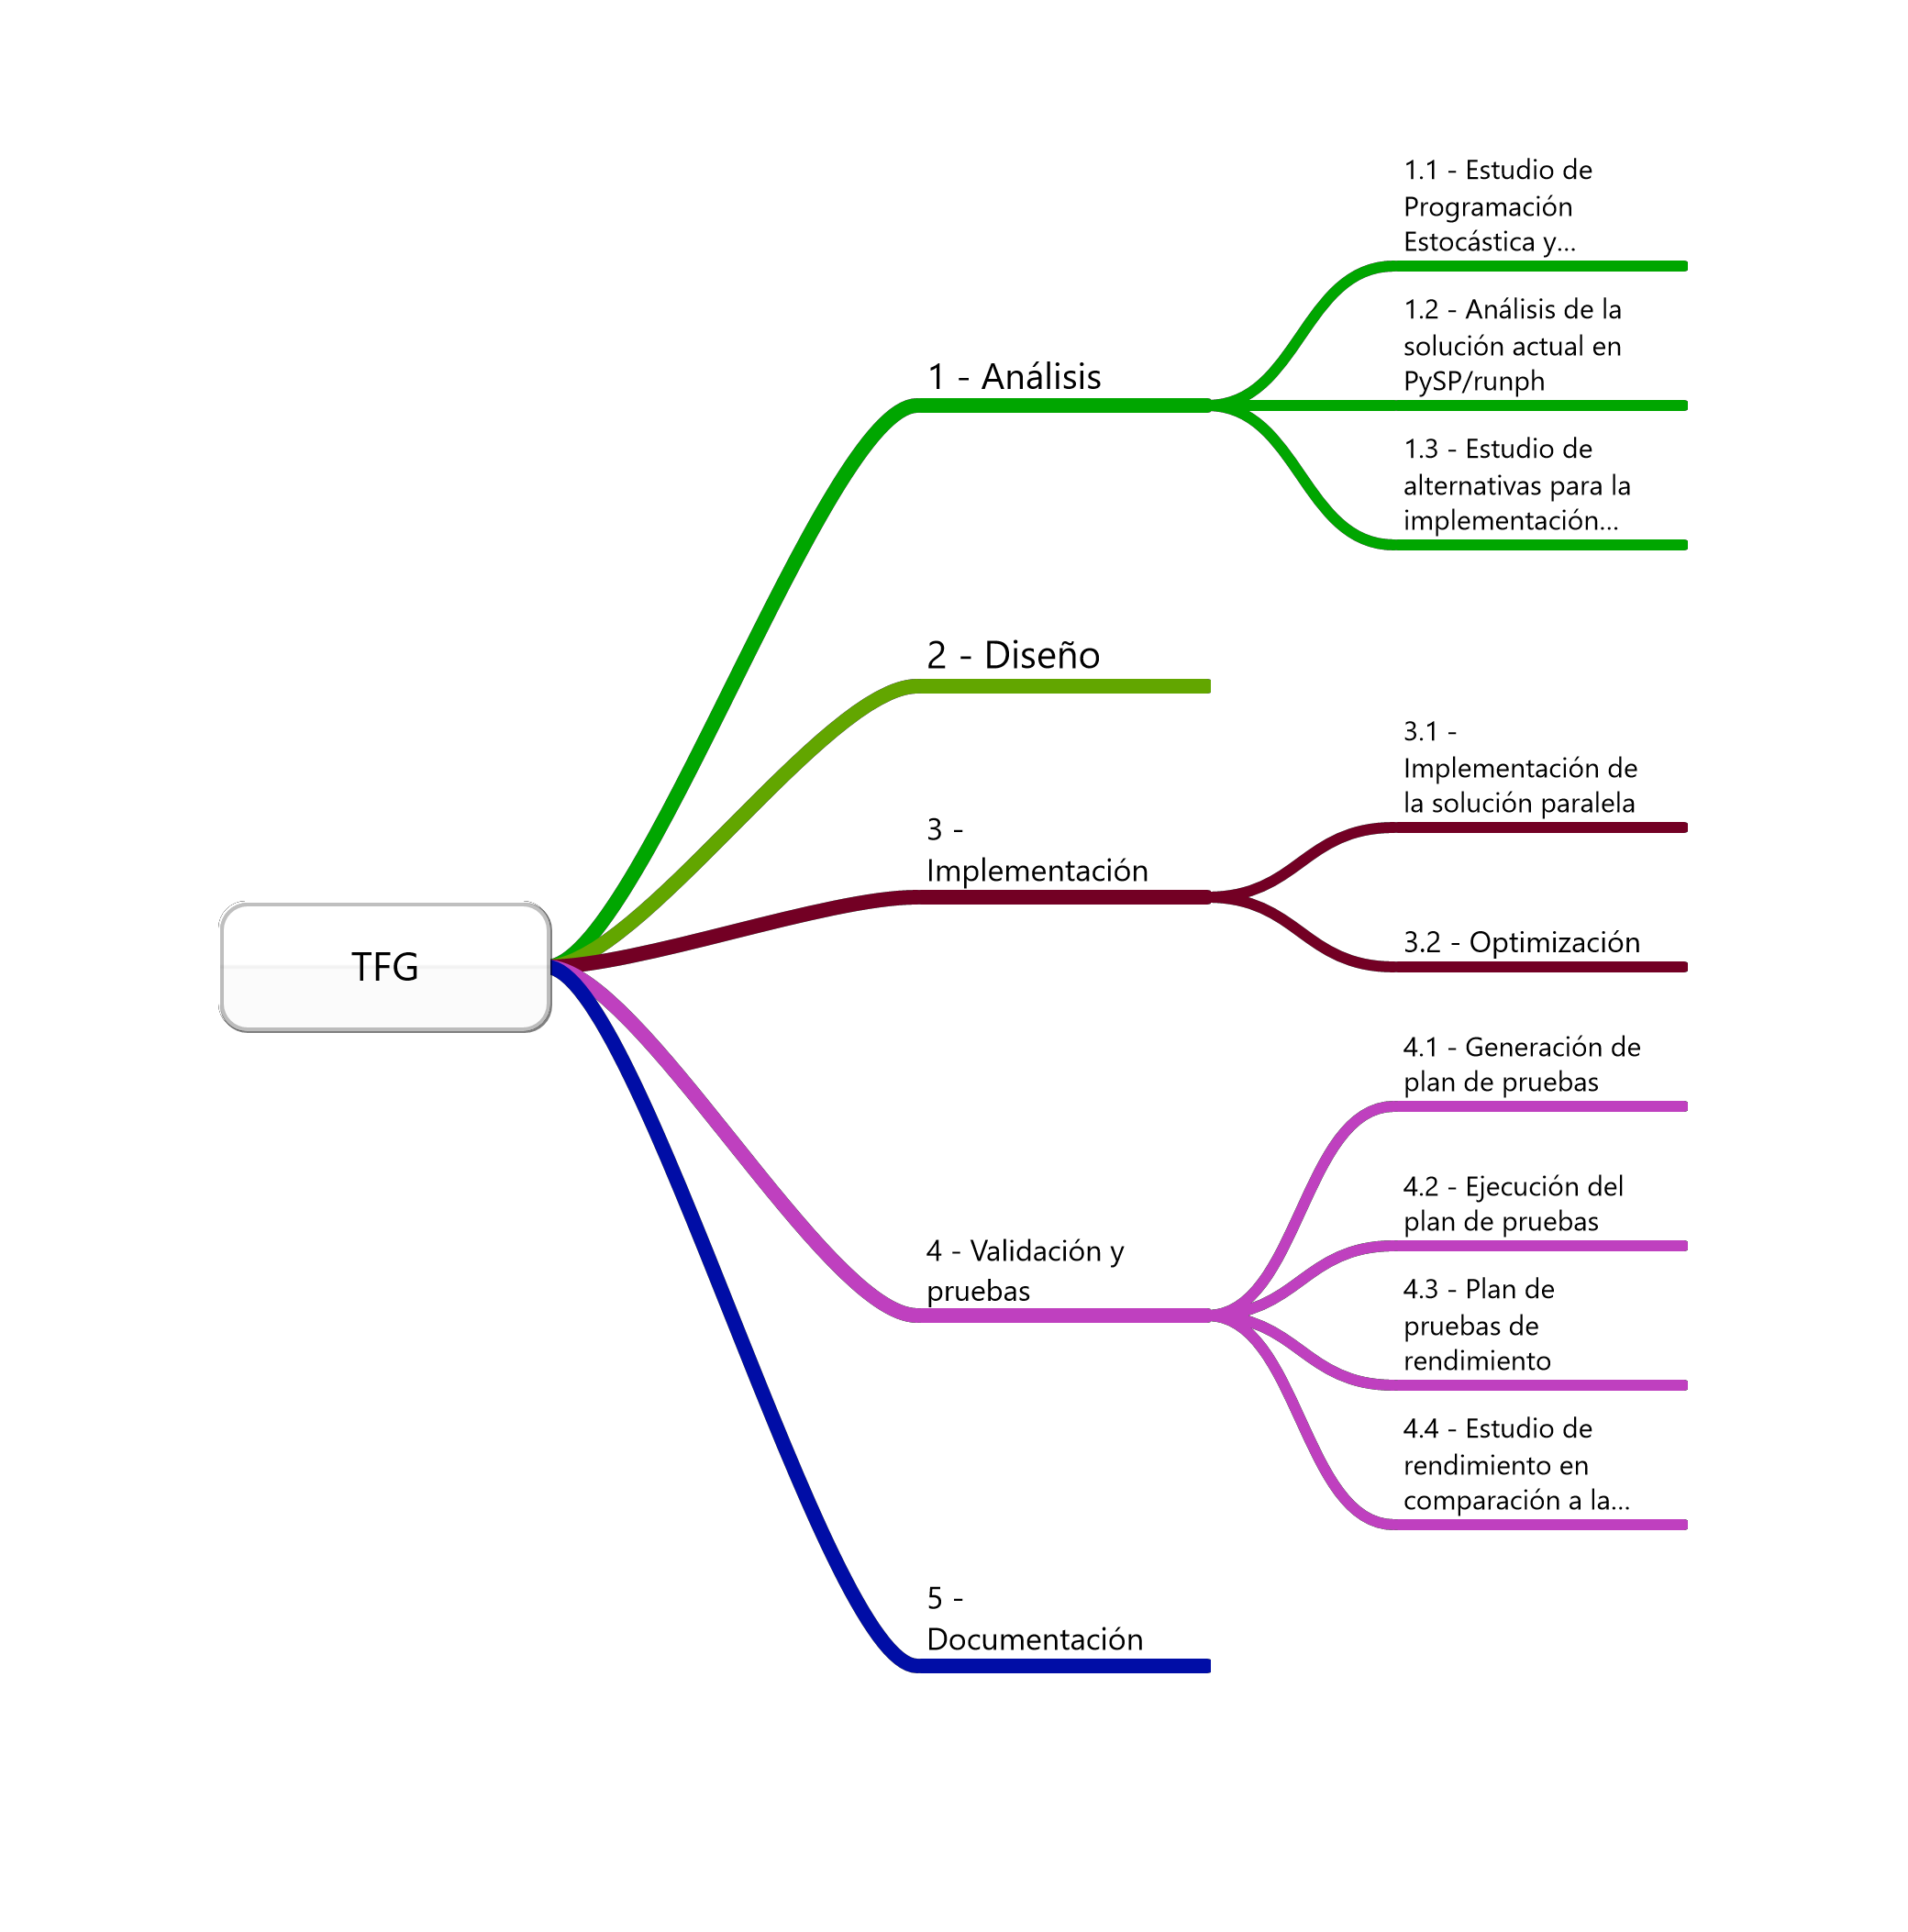
\includegraphics[width=15cm]{figuras/planificacion/edt-inicial.png}}
    \caption{EDT inicial}
\end{figure}

\WorkItem [
            id=1.1, 
            name={Estudio de Programación Estocástica y Progressive Hedging},
            duration=7,
            results={N/A}
        ]
{
    Se investigará el funcionamiento del algoritmo {\it Progressive Hedging} haciendo uso principalmente de \cite{stochasticProgramming} como referencia.
}

\WorkItem [
        id=1.2, 
        name={Análisis de la solución actual en PySP/runph},
        duration=8,
        results={Diagrama de funcionamiento PH \cite{local_funcionamientoPH}.}
    ]
{
    Una vez conocido el funcionamiento teórico del algoritmo, estudiar su implementación sobre el proyecto Pyomo.
}

\WorkItem [
        id=1.3, 
        name={Estudio de alternativas para la implementación paralela},
        duration=3,
        results={TODO}
    ]
{
    Se barajarán tecnologías Big Data (Spark) o modelos tradicionales (MPI).
}

\WorkItem [
        id=2, 
        name={Diseño},
        duration=20,
        results={Diseño de la implementación.}
    ]
{
    Generar un diseño de la implementación a realizar con la tecnología escogida. Será importante la integración con la implementación actual.
}

\WorkItem [
        id=3.1, 
        name={Implementación de la solución paralela},
        duration=15,
        results={Nuevos ficheros de código y modificaciones a archivos existentes.}
    ]
{
    Escribir los nuevos módulos de código e integrarlos en el proyecto. 
}

\WorkItem [
        id=3.2, 
        name={Optimización},
        duration=5,
        results={Modificaciones a la implementación anterior.}
    ]
{
    Una vez la integración es correcta y la implementación funciona, se realizarán optimizaciones de rendimiento intentando aprovechar las carácterísticas de la tecnología escogida para la nueva implementación paralela.
}

\WorkItem [
        id=4.1, 
        name={Generación de plan de pruebas},
        duration=4,
        results={Documento de pruebas \cite{local_planPruebas}.}
    ]
{
    Idear un plan de pruebas para el nuevo módulo.
}

\WorkItem [
        id=4.2, 
        name={Ejecución del plan de pruebas},
        duration=1,
        results={Informe de ejecución de pruebas.}
    ]
{
    Implementar y ejecutar las pruebas establecidas para establecer confianza sobre el correcto funcionamiento de la implementación.
}

\WorkItem [
        id=4.3, 
        name={Plan de pruebas de rendimiento},
        duration=3,
        results={Documento de pruebas de rendimiento \cite{local_planPruebasRendimiento}.}
    ]
{
    Idear un plan de pruebas con problemas que permitan estudiar el rendimiento del programa.
}

\WorkItem [
        id=4.4, 
        name={Estudio de rendimiento},
        duration=2,
        results={Informe de rendimiento \cite{local_informeRendimiento}.}
    ]
{
    Ejecutar el plan de pruebas anterior y compararlo con las versiones originales tanto secuencial como con Pyro.
}



\WorkItem [
        id=5, 
        name={Documentación},
        duration=10,
        results={Memoria del proyecto y documentos asociados.}
    ]
{
    Generar los documentos asociados al desarrollo del proyecto.
}

\subsubsection{Tareas no planificadas}

Tras las modificaciones realizadas sobre el cronograma y explicadas en \autoref{sec:modificacionesCronograma}, se generan nuevas tareas para el proyecto: 
 
\WorkItem [ 
        id=3.*,  
        name={Prototipo aislado}, 
        duration=10, 
        results={Proyecto de pruebas en Python \cite{local_distributedTestApp}.} 
    ] 
{ 
    Crear una aplicación en Python que interactúe con Spark de forma similar a como lo hará la implementación en Pyomo. 
} 
 
\WorkItem [ 
        id=3.*,  
        name={Prototipo de integración inicial}, 
        duration=5, 
        results={Código añadido a Pyomo.} 
    ] 
{ 
    Comenzar la implementación sobre Pyomo comprobando que la integración del nuevo módulo con el código existente es correcta y el flujo de ejecución es correcto con respecto al funcionamiento anterior. 
} 
 
\WorkItem [ 
        id=3.*,  
        name={Prototipo funcional}, 
        duration=10, 
        results={Código añadido a Pyomo.} 
    ] 
{ 
    Modificar el prototipo anterior añadiendo las funcionalidades esperadas del programa. 
} 

\subsection{Cronograma inicial}

Para la realización del trabajo se plantea un ciclo de vida en cascada. Este ciclo de vida nos permitirá realizar un seguimiento del progreso del proyecto en función del tiempo disponible.

\begin{figure}[H]
    \centerline{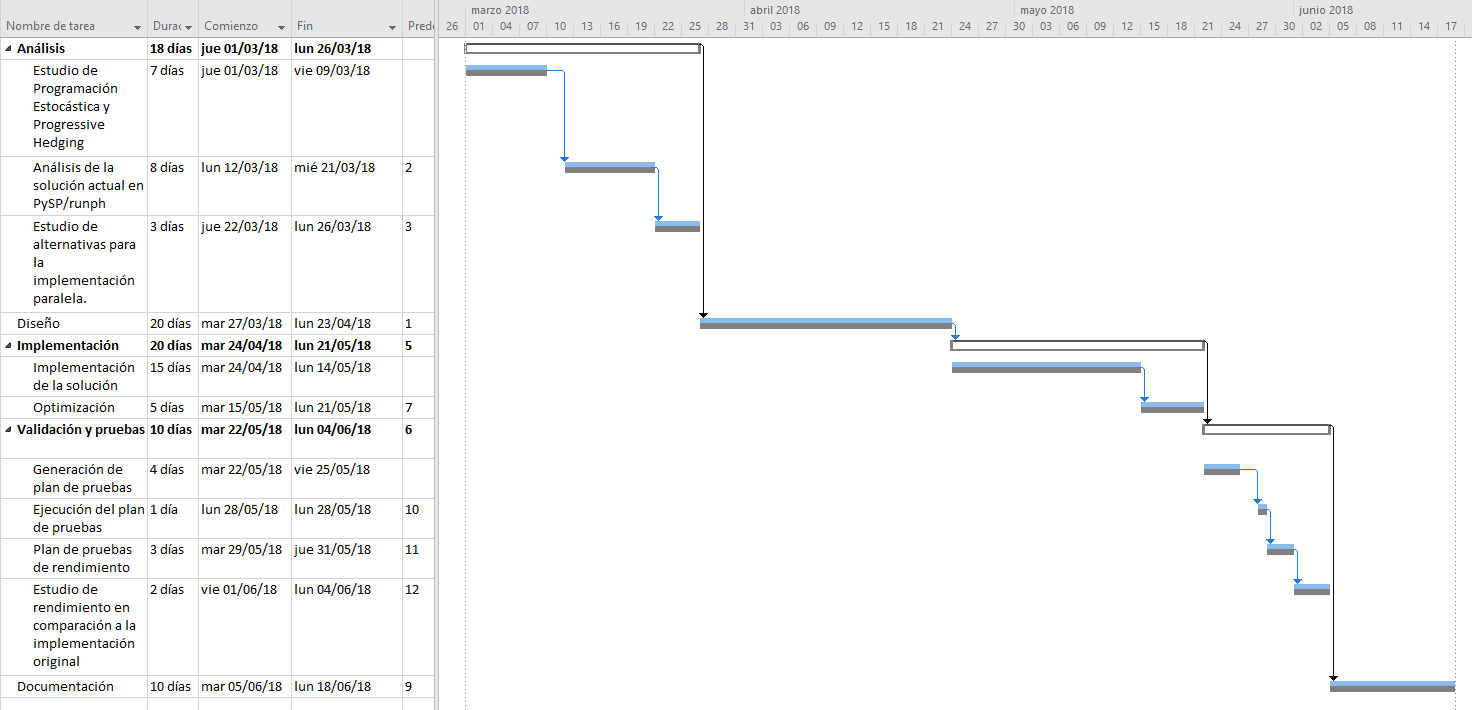
\includegraphics[width=15cm]{figuras/planificacion/linea-base.png}}
    \caption{Línea base}
\end{figure}

\subsection{Modificaciones al cronograma inicial}
\label{sec:modificacionesCronograma}

Se ha realizado una estimación temporal inicial poco precisa por no utilizar ningún tipo de método probado ni datos concretos.

Esta es la razón principal para los retrasos que se explican a continuación.

\subsubsection{Retraso en análisis}

El primer retraso se produce en la fase de análisis de la implementación actual. En esta fase se debe estudiar el funcionamiento del proyecto Pyomo y, en concreto, el módulo de resolución de problemas mediante Progressive Hedging. 

A pesar de conocer el funcionamiento teórico del algoritmo mediante \cite{TODO}, Pyomo es un proyecto complejo, con multitud de funcionalidades para resolver otros tipos de problemas, soporte para plugins, etc. Todo esto hace que la complejidad del código aumente y sea necesario estudiar múltiples capas de abstracción para entender correctamente el funcionamiento del programa.

Otra complicación añadida es el personal desconocimiento del lenguaje Python previo a la realización de este trabajo.\\

Tras este primer retraso se intenta ajustar la planificación reduciendo el tiempo de diseño a la mitad:

\begin{figure}[H]
    \centerline{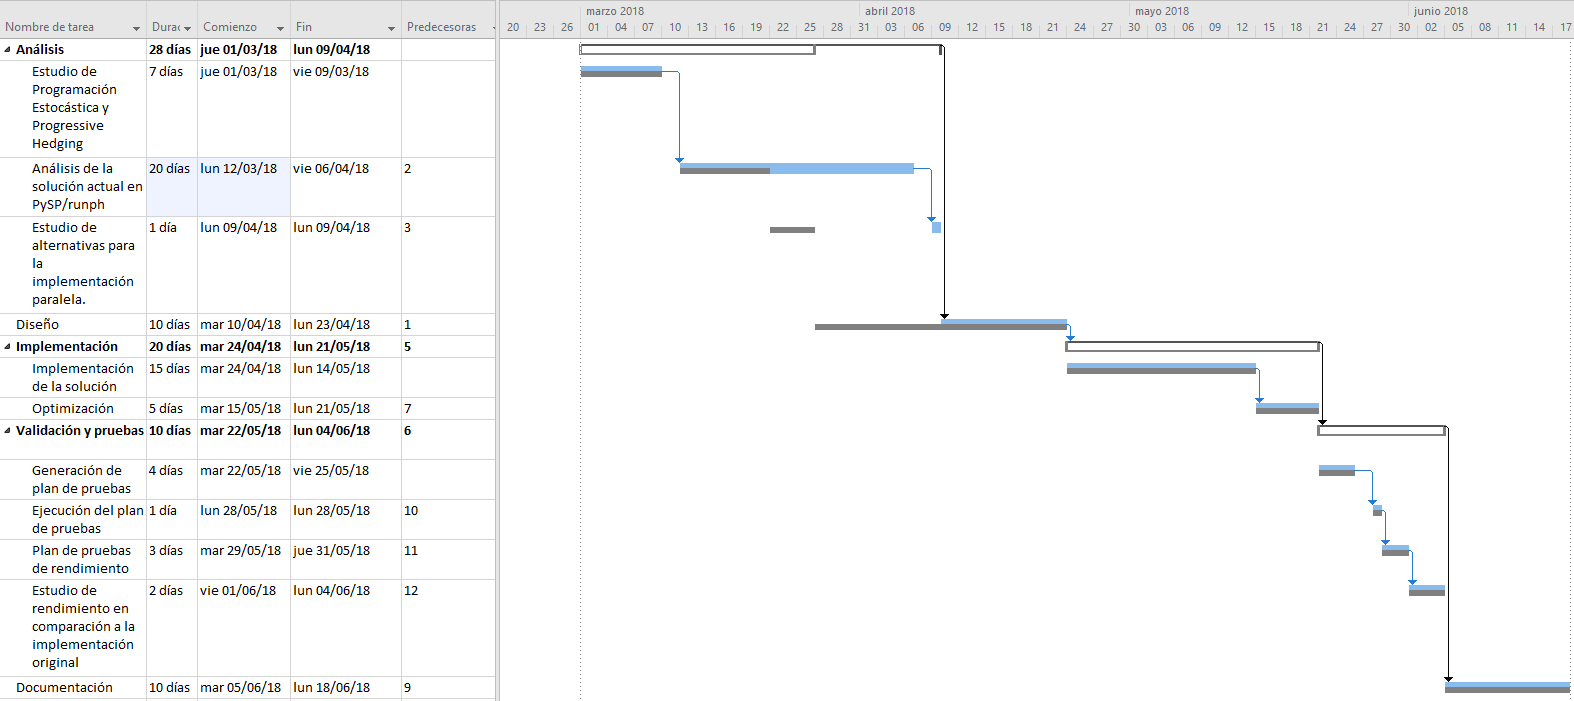
\includegraphics[width=15cm]{figuras/planificacion/1_retraso-analisis-inicial.png}}
    \caption{Primer retraso}
\end{figure}

Teniendo en cuenta que los primeros retrasos fueron principalmente causados por el desconocimiento de la tecnología a usar así como de una mala estimación, es muy probable que en las fases siguientes se produzcan otros retrasos. En este punto se considera entonces abandonar el ciclo de vida en cascada. Su principal atractivo era poder ajustarnos a una planificación temporal que nos permita acabar el proyecto dentro de tiempo, pero esta ventaja no se está cumpliendo en la práctica. Buscando reducir el tiempo de implementación con tecnologías que serán usadas por primera vez, se decide adaptar la planificación a un ciclo de vida por prototipos. 

La creación de sucesivos prototipos permite ir acostumbrándose a las tecnologías desconocidas, en este caso Python y Spark, así como ir probando el rendimiento y la integración a medida que se desarrolla.

En primer lugar se crea un prototipo aislado para comprobar la implementación de Spark con una arquitectura similar a la que se implementará en Pyomo. Este primer prototipo sirve como aprendizaje de la instalación de Spark y el despliegue de una aplicación en el mismo, así como la implementación en python que interactuará con Spark. Es deseable utilizar una arquitectura de objetos python similar a la que se usará en Pyomo para concretar el uso de Spark y descubrir posibles problemas con la implementación elegida.

Posteriormente se realizarán prototipos sucesivos sobre Pyomo para integrar el nuevo módulo e ir solucionando posibles problemas de rendimiento o funcionamiento que vayan surgiendo. 

Dado que la implementación partirá de un protipo inicial de baja calidad será importante realizar una fase de optimización y refactorización al final de la implementación para asegurarse un código final de calidad. Definir la calidad del código no es algo trivial y en este caso calificaremos el código como "de calidad" si cumple:
% TODO: meter mierdas de calidad de software y si eso alguna ISO

\begin{itemize}
    \item Funciona correctamente y es resistente a errores. Para esto nos apoyaremos en un plan de pruebas funcional.
    \item Funciona eficientemente y otorga un buen rendimiento, en comparación a las implementaciones existentes. En este caso nos apoyaremos en el plan de pruebas de rendimiento.
    \item Se integra adecuadamente al proyecto actual. Debe seguir una filosofía de diseño análoga al resto del código así como funcionar correctamente de forma paralela a todo lo implementado previamente.
\end{itemize}

Tras esta modificación en la planificación, se genera una nueva planificación que podemos ver en la figura y se guardará como una nueva línea base.% TODO

\begin{figure}[H]
    \centerline{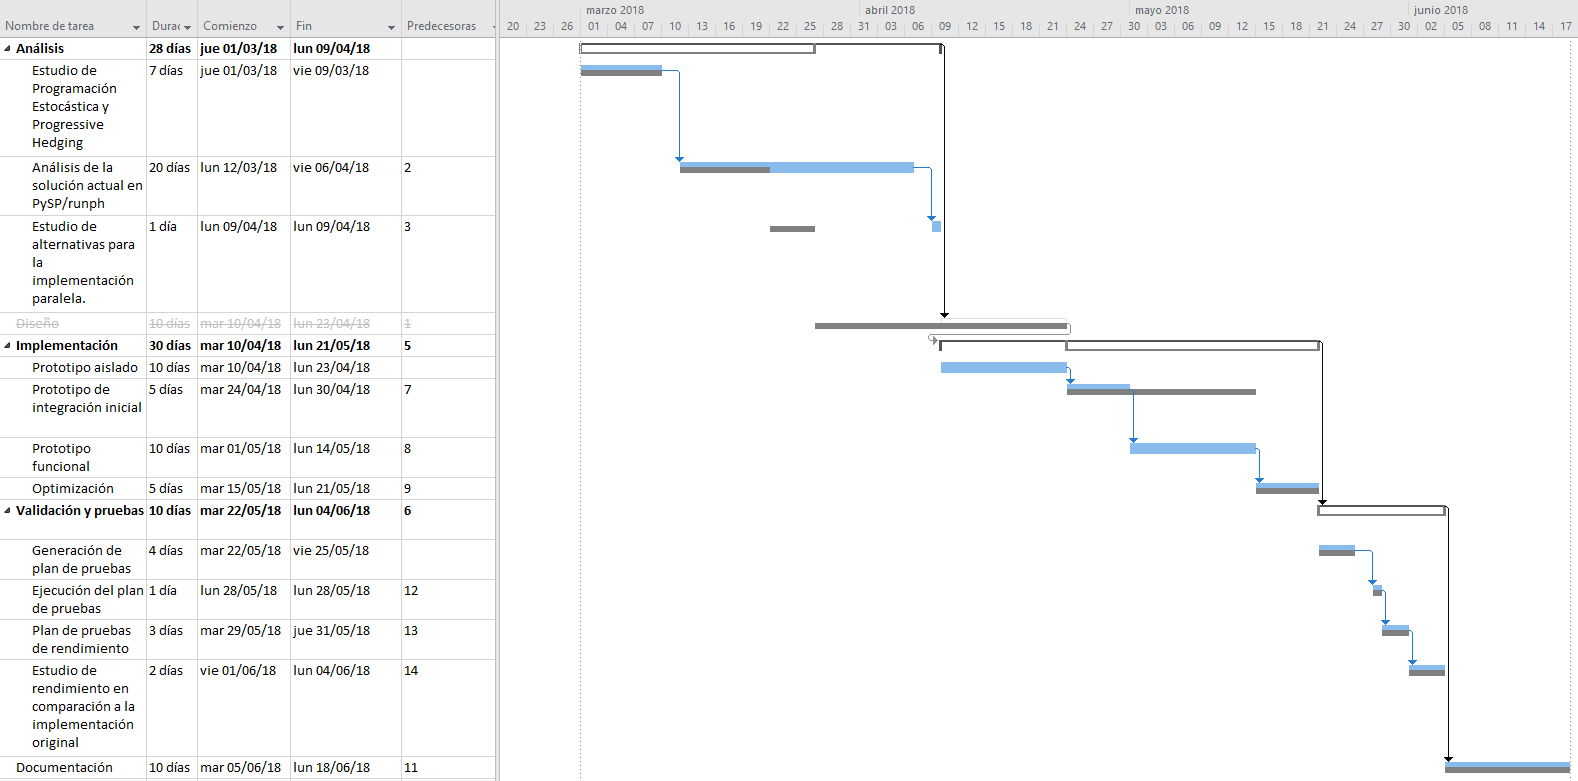
\includegraphics[width=15cm]{figuras/planificacion/2_linea-base-prototipos.png}}
    \caption{Línea base prototipos}
\end{figure}

En este punto hemos eliminado la fase de Diseño para poder aumentar el tiempo asignado a Análisis e Implementación. En caso de sufrir más retrasos en la fase de implementación podremos reducir el tiempo asignado a pruebas si el retraso no es grave. En caso de ser un retraso mayor, no cumpliremos la fecha de finalización establecida.

\subsubsection{Retraso en implementación}

Durante la implementación del prototipo funcional el desarrollo llega a un punto muerto. Las funciones implementadas no devuelven el resultado correcto y se debe hacer una búsqueda de los errores que lo causan. Por falta de experiencia y desconocimiento de las tecnologías, esta fase de implementación se alarga hasta el día 07/07/2018. \\

Este retraso sumado a un retraso de 10 días en la creación del prototipo aislado nos fuerza a retrasar la fecha de finalización del proyecto al día 25/07/2018. \\

Con estos nuevos cambios es necesaria una nueva planificación temporal:

\begin{figure}[H]
    \centerline{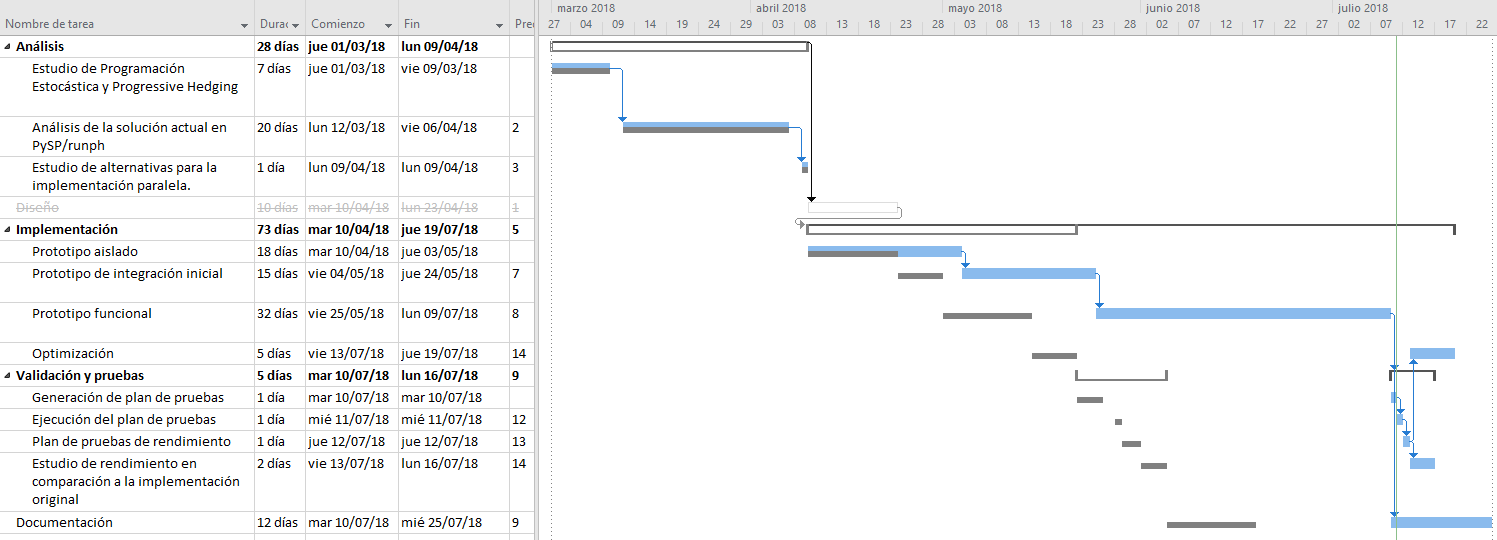
\includegraphics[width=15cm]{figuras/planificacion/3_linea-base-final.png}}
    \caption{Línea base final}
\end{figure}

